
%%
%% This is file `sample-sigconf-authordraft.tex',
%% generated with the docstrip utility.
%%
%% The original source files were:
%%
%% samples.dtx  (with options: `all,proceedings,bibtex,authordraft')
%% 
%% IMPORTANT NOTICE:
%% 
%% For the copyright see the source file.
%% 
%% Any modified versions of this file must be renamed
%% with new filenames distinct from sample-sigconf-authordraft.tex.
%% 
%% For distribution of the original source see the terms
%% for copying and modification in the file samples.dtx.
%% 
%% This generated file may be distributed as long as the
%% original source files, as listed above, are part of the
%% same distribution. (The sources need not necessarily be
%% in the same archive or directory.)
%%
%%
%% Commands for TeXCount
%TC:macro \cite [option:text,text]
%TC:macro \citep [option:text,text]
%TC:macro \citet [option:text,text]
%TC:envir table 0 1
%TC:envir table* 0 1
%TC:envir tabular [ignore] word
%TC:envir displaymath 0 word
%TC:envir math 0 word
%TC:envir comment 0 0
%%
%% The first command in your LaTeX source must be the \documentclass
%% command.
%%
%% For submission and review of your manuscript please change the
%% command to \documentclass[manuscript, screen, review]{acmart}.
%%
%% When submitting camera ready or to TAPS, please change the command
%% to \documentclass[sigconf]{acmart} or whichever template is required
%% for your publication.
%%
%%
\documentclass[conference]{IEEEtran}
\IEEEoverridecommandlockouts  % only needed if you use \thanks for funding in the first footnote
\bibliographystyle{IEEEtran}
\usepackage{cite}
\usepackage{amsmath,amssymb,amsfonts}
\usepackage{hyperref} 
\usepackage{graphicx}
\usepackage[utf8]{inputenc}
\usepackage{textcomp}
\usepackage{enumitem}
\usepackage{booktabs}
\usepackage{multirow}
\usepackage{xcolor}      % must precede \definecolor and \textcolor usage
\usepackage{colortbl}
\usepackage{tcolorbox}
\tcbuselibrary{skins}
\newcommand{\BJohnson}[1]{\textcolor{purple}{{\bfseries [[#1]]}}}
\newcommand{\EAdejumo}[1]{\textcolor{red}{{\bfseries [[#1]]}}}
\newcommand{\MGuizani}[1]{\textcolor{blue}{{\bfseries [[#1]]}}}
\usepackage{enumitem}
\usepackage{booktabs}
\usepackage[utf8]{inputenc}
\usepackage{textcomp}
\definecolor{heatmaplight}{HTML}{DBEAFE}
\definecolor{heatmapdark}{HTML}{1F4E79}
\usepackage{multirow}
\usepackage{tcolorbox}
\tcbuselibrary{skins}
\usepackage{colortbl}
\usepackage{xcolor}
\newenvironment{observation}{%
  \begin{tcolorbox}[
    colback=gray!6,
    colframe=gray!40,
    boxrule=0.5pt,
    arc=2pt,
    left=6pt, right=6pt,
    top=4pt, bottom=4pt,
    fontupper=\small
  ]
}{%
  \end{tcolorbox}
}



%%
%% Submission ID.
%% Use this when submitting an article to a sponsored event. You'll
%% receive a unique submission ID from the organizers
%% of the event, and this ID should be used as the parameter to this command.
%%\acmSubmissionID{123-A56-BU3}

%%
%% For managing citations, it is recommended to use bibliography
%% files in BibTeX format.
%%
%% You can then either use BibTeX with the ACM-Reference-Format style,
%% or BibLaTeX with the acmnumeric or acmauthoryear sytles, that include
%% support for advanced citation of software artefact from the
%% biblatex-software package, also separately available on CTAN.
%%
%% Look at the sample-*-biblatex.tex files for templates showcasing
%% the biblatex styles.
%%

%%
%% The majority of ACM publications use numbered citations and
%% references.  The command \citestyle{authoryear} switches to the
%% "author year" style.
%%
%% If you are preparing content for an event
%% sponsored by ACM SIGGRAPH, you must use the "author year" style of
%% citations and references.
%% Uncommenting
%% the next command will enable that style.
%%\citestyle{acmauthoryear}


%%
%% end of the preamble, start of the body of the document source.
\begin{document}

\title{When Deliberation Stalls: Engagement, Affect, and Governance Debt in Rust RFCs}

% \author{
% \IEEEauthorblockN{Elijah Kayode Adejumo\IEEEauthorrefmark{1}, Matteo Vaccargiu\IEEEauthorrefmark{2}, Brittany Johnson\IEEEauthorrefmark{1}}
% \IEEEauthorblockA{\IEEEauthorrefmark{1}Department of Computer Science, George Mason University, Fairfax, VA, USA\\
% Email: eadejumo@gmu.edu, johnsonb@gmu.edu}
% \IEEEauthorblockA{\IEEEauthorrefmark{2}University of Hohenheim, Stuttgart, Germany\\
% Email: matteo.vaccargiu@uni-hohenheim.de}
% }
\maketitle

\begin{abstract}
Open source projects settle their direction through deliberation: a design proposal is submitted, discussed in public, and eventually accepted, rejected, or postponed. Studies of these processes have treated outcomes as adoption or decline, leaving postponement unexamined. We analyze 1,469 proposals to Rust's Request-for-Comments (RFC) process (2014--2026) and their 57,108 comments. Accepted proposals draw broader and more established participation than rejected ones and a markedly less negative discussion tone ($r = 0.481$); tone remains the strongest difference when the same author's accepted and rejected proposals are compared ($r = 0.738$). Postponed proposals form a distinct profile. They attract as much discussion and as many established participants as accepted proposals, and more than rejected ones, yet their tone resembles that of rejected proposals and their discussions carry the most confusion of the three groups. We call this state \emph{governance debt}: deliberation that absorbs community attention without converging on a decision. Its signature appears early. Among proposals still undecided 30 days after submission, those later postponed already show more participation than those later rejected and more confusion than those later accepted, while confusion does not separate eventual acceptance from rejection. Stalled deliberation may therefore be detectable while it can still be addressed.
\end{abstract}

\section{Introduction}
Open source software (OSS) projects decide what their software will become through deliberation. In formal proposal processes such as Python Enhancement Proposals (PEPs), Kubernetes Enhancement Proposals (KEPs), and Rust's Requests for Comments (RFCs), a contributor writes a design proposal, the community discusses it in public, and a team eventually accepts, rejects, or postpones it~\cite{9402135, https://doi.org/10.1002/spe.3128}. These decisions bind a language or platform for years and are hard to reverse, which makes the deliberation behind them a central socio-technical process~\cite{lambiase2024cultural}.

Research on how OSS communities decide has examined the rationale behind decisions in Python's mailing lists and PEPs~\cite{9402135, https://doi.org/10.1002/spe.3128, sharma2024decisions}, why Go proposals are declined~\cite{kondo2025empirical}, how ecosystems negotiate the cost of breaking changes~\cite{bogart2016break}, how teams discuss tool adoption~\cite{yin2020team}, and how architectural decisions surface in mailing lists~\cite{soliman2024exploring}. Pull-request studies show that acceptance depends on social as well as technical factors~\cite{tsay2014influence, gousios2015work}, and research on affect shows that the emotional tone of developer communication relates to process outcomes~\cite{murgia2014developers, ortu2015bullies, novielli2019sentiment}. Across this literature, a decision has two outcomes: a proposal is adopted or it is not.

Formal processes have a third outcome. A postponed proposal is neither accepted nor rejected: the community has invested in deliberating it, no decision has been reached, and the question returns later. In Rust, postponed proposals stayed open for a median of 135 days before being deferred, against 55 days for accepted and 49 days for rejected proposals, and a quarter of them stayed open for more than 19 months. We call this unresolved deliberation \emph{governance debt}, by analogy with technical and social debt~\cite{tamburri2013social}: effort is spent now, the decision is deferred, and its cost is carried forward. If governance debt has a recognizable signature, maintainers could spot stalling discussions while they can still be steered.

We study governance debt in the Rust RFC process, the formal path through which significant changes to Rust are proposed, debated, and decided. The process is meant to provide ``a consistent and controlled path for changes to Rust such that all stakeholders can be confident about the direction of the project''~\cite{RustRFC2024}, and its complete record is public. We examine each discussion through two lenses: \emph{engagement}, meaning how many people take part and how established they are in the community, and \emph{affect}, meaning the tone and emotions expressed in the comments. No single measure separates all three outcomes, which is why we combine them. We ask:

\begin{description}
    \item[\textbf{RQ$_1$}] \textit{How do engagement and affect differ across accepted, rejected, and postponed RFCs?}
    \item[\textbf{RQ$_2$}] \textit{Is the signature of postponement visible early in deliberation?}
\end{description}

Our findings separate three outcomes rather than two. Accepted proposals draw broader and more established participation and a markedly less negative tone than rejected ones, and both differences hold when the same author's accepted and rejected proposals are compared. Tone is the more robust of the two: it persists even for proposals by the same author submitted about two months apart, whereas the engagement differences weaken, suggesting that how a discussion sounds tracks its outcome more consistently than who joins it (RQ$_1$). For postponed proposals, engagement and tone point in different directions. Their engagement looks like that of accepted proposals: they draw exactly as many commenters, although fewer of them are core members. Their tone looks like that of rejected proposals. They also show the most confusion of the three groups. Confusion does not separate accepted from rejected proposals; it points to discussions that stall, not to proposals that get rejected. Some of these signs, namely more engagement than rejected proposals and more confusion than accepted ones, already appear within 30 days of submission, months before a typical postponed proposal is closed (RQ$_2$).

Our contributions are: (1) a three-outcome characterization of deliberative governance that separates postponement from rejection, built on formally defined engagement metrics that can be reused for other proposal processes; (2) the concept of governance debt, deliberation that absorbs community attention without producing a decision, together with an early signature that maintainers could use to spot stalling discussions; and (3) a replication package with data and scripts~\cite{rrgc2026}.

\section{Related Work}
\textbf{Decision-making in OSS proposal processes.} Sharma et al.\ extracted decision rationale from Python's email archives~\cite{9402135}, reconstructed how PEP decisions are made~\cite{https://doi.org/10.1002/spe.3128}, and studied how rationale is expressed in Python decision discussions~\cite{sharma2024decisions}. Kondo et al.\ analyzed why Go proposals are declined and how early their outcome can be predicted~\cite{kondo2025empirical}. Bogart et al.\ showed how three ecosystems negotiate the cost of breaking changes according to their community values~\cite{bogart2016break}, Yin and Filkov examined team discussions during DevOps tool adoption~\cite{yin2020team}, and Soliman traced architectural design decisions from mailing lists to issue trackers~\cite{soliman2024exploring}. These studies explain what is decided and why, largely through the content of discussions, and treat outcomes as adoption or decline. We quantify process signals, namely who participates and how they express themselves, across three outcomes, separate postponement from rejection, and test when the signature of postponement becomes visible.

\textbf{Social factors in contribution acceptance.} Pull-request studies show that contributor reputation, social connections, and prior interaction shape acceptance alongside code quality~\cite{tsay2014influence, gousios2014dataset, gousios2015work, dey2020effect, iyer2019effects}. OSS communities follow a core-periphery structure in which a small core holds disproportionate influence~\cite{crowston2005social, crowston2006hierarchy, steinmacher2015social}. We measure participants' standing at the time each proposal is submitted and hold author identity constant with within-author comparisons.

\textbf{Affect in software engineering.} Emotions are detectable in software artifacts and relate to issue resolution time, question answering, and communication quality~\cite{murgia2014developers, ortu2015bullies, calefato2018ask, islam2018sentistrength}. This work has focused on issues, code review, and Q\&A, and has shown that general-purpose sentiment tools can misread technical text~\cite{novielli2019sentiment}. We extend affect analysis to extended governance deliberation.

\textbf{Debt and governance.} Technical debt describes deferred engineering work; social debt describes the cost created by suboptimal social and organizational structures in development communities~\cite{tamburri2013social}. Governance research has examined OSS governance documents, institutions, and contributor roles~\cite{yin2022open, yan2023github, gerosa2021shifting, trinkenreich2020hidden}. Governance debt differs from social debt in its unit: it attaches to an individual proposal in a formal decision process and can be observed in that proposal's discussion.

\section{Methodology}

\subsection{Data and Outcome Labels}
We cloned the Rust RFC repository, in which every proposal is submitted as a pull request (PR), and collected all PR comments through the GitHub REST API. A merged PR is labeled \emph{accepted}, a closed PR with the repository's \texttt{postponed} label is labeled \emph{postponed}, and any other closed PR is labeled \emph{rejected}. We excluded 18 PRs withdrawn by their authors, 36 PRs labeled \texttt{not-rfc} or \texttt{april-1st}, three PRs whose final-comment-period disposition label contradicts their outcome (e.g., a closed PR labeled \texttt{disposition-merge}), and 15 accepted RFCs whose PR lacks creation or merge dates; one PR that introduced two RFCs is counted once. The final corpus contains 1,469 proposals submitted between March 2014 and March 2026 (609 accepted, 758 rejected, 102 postponed) with 57,108 comments by 2,209 people. Comments by bots (\texttt{rfcbot}, \texttt{rust-highfive}, \texttt{bors}, \texttt{bors-servo}, \texttt{rust-rfcbot}, \texttt{rustbot}, and \texttt{renovate[bot]}) were removed.

\subsection{Engagement Metrics}
OSS projects are frequently characterized as meritocracies, in which contribution decisions are driven by technical quality. Tsay et al.~\cite{tsay2014influence} challenged this assumption, demonstrating that social factors, including the contributor's activity history, predict whether a contribution is accepted independently of its technical merit. Social barriers that prevent newcomers from making their first contribution have also been studied in detail~\cite{steinmacher2015social}. These findings suggest that open source, commonly portrayed as a meritocracy~\cite{kondo2025empirical}, has a complex social structure beneath it, which motivates the study of engagement dynamics.

To support precise interpretation and reuse, we give each engagement metric a description and a formal definition, each grounded in established network constructs~\cite{freeman1978centrality, crowston2006hierarchy}. Let $\mathcal{R}$ denote the corpus of 1,469 RFC proposals. For proposal $r \in \mathcal{R}$ submitted at time $t_r$, let $C(r) = \langle c_1, c_2, \ldots, c_n \rangle$ denote the time-ordered sequence of human comments on proposal $r$ (for RQ$_2$, those posted in an early window), and let $\tilde{C}(r)$ denote the set of their authors. For each participant $p$, we define their prospective network degree $d_t(p)$ as the number of distinct proposals they had commented on before time $t$:
\begin{equation}
  d_t(p) = \left|\{r' \in \mathcal{R} : p \text{ commented on } r' \text{ before } t\}\right|
  \label{eq:degree}
\end{equation}
Counting only earlier comments ensures that a participant's degree reflects their governance standing at the time of deliberation and that later activity does not leak into the measure.

\textbf{Review Duration} measures the time from RFC submission to the final governance decision: the number of calendar days between the PR's creation and either its merge (accepted proposals) or its close (rejected and postponed proposals).

\textbf{Unique Commenters} counts the distinct human participants who commented on a proposal. It operationalizes the breadth of community engagement, that is, how many distinct voices a proposal drew into the discussion: $\text{UC}(r) = |\tilde{C}(r)|$. We also report the number of comments, $|C(r)|$.

\textbf{Influence Score} is the sum of the prospective network degrees of a proposal's unique commenters. Degree centrality is a foundational measure of network influence~\cite{freeman1978centrality, wasserman1994social}, operationalized here as participation volume following Crowston and Howison's approach to measuring hierarchy in OSS communication networks~\cite{crowston2006hierarchy}:
\begin{equation}
  \text{INF}(r) = \sum_{p \,\in\, \tilde{C}(r)} d_{t_r}(p)
  \label{eq:inf}
\end{equation}
A commenter who had participated in many RFC discussions before the proposal contributes more to $\text{INF}(r)$ than one who had participated in few.

\textbf{Echo Score} is the fraction of a proposal's commenters who belong to the governance core, the most active participants in RFC discussions. To set the size of this core empirically, we first calculated the median number of unique commenters per proposal in our corpus (Mdn\,=\,10) and used it as the threshold: the governance core $\mathcal{G}_{t_r}$ consists of the $k = 10$ participants with the highest prospective network degree at the time proposal $r$ is submitted. We define the core at submission time, rather than over the whole corpus, so that a participant's future activity cannot make them a core member for earlier proposals. Across the corpus, the ten participants who commented on the most proposals make up 0.45\% of the 2,209 participants yet account for 17.9\% of all participation (person--proposal pairs), the core-periphery structure typical of OSS communication networks~\cite{crowston2005social}.

Echo Score operationalizes the degree to which a proposal attracted insider engagement: a score of 0 indicates that no core member commented, and a score of 1 that every commenter was a core member:
\begin{equation}
  \text{ECHO}(r) =
  \begin{cases}
    \dfrac{|\tilde{C}(r) \cap \mathcal{G}_{t_r}|}{|\tilde{C}(r)|} & \text{if } \tilde{C}(r) \neq \emptyset \\[8pt]
    0 & \text{otherwise}
  \end{cases}
  \label{eq:echo}
\end{equation}

\textbf{First Commenter Degree} is the prospective network degree of the first person to comment on a proposal. It operationalizes the authority of the opening voice, the participant who frames the initial direction of the discussion. The significance of first responses in OSS contribution processes is established~\cite{assavakamhaenghan2023does, yue2022off}, and we test whether the centrality of the first commenter carries signal beyond that of the broader commenter pool:
\begin{equation}
  \text{FCD}(r) = d_{t_r}(p_1)
  \label{eq:fcd}
\end{equation}
where $p_1$ is the author of $c_1$, the earliest comment in $C(r)$.

\subsection{Affect Metrics}
RFC discussions are extended deliberative exchanges in which community members express enthusiasm, raise concerns, signal confusion, and register approval or disapproval over days, weeks, and sometimes months before a governance decision is reached. We characterize their emotional dynamics with two complementary NLP pipelines applied to every comment.

\textbf{Sentiment Analysis:} We apply SiEBERT (\texttt{siebert/sentiment-roberta-large-english})~\cite{hartmann2023more}, a RoBERTa-large sentiment classifier that its authors fine-tuned on 15 datasets spanning diverse domains, resulting in strong generalization; we use it as published, without further training. The model assigns each comment $c$ a sentiment score $s(c) = P(\text{positive}) - P(\text{negative}) \in [-1, +1]$. We define the \textbf{Governance Tone Trajectory (GTT)} of proposal $r$ as the mean sentiment score across its comments:
\begin{equation}
  \text{GTT}(r) = \frac{1}{|C(r)|}
  \sum_{c \,\in\, C(r)} s(c)
  \label{eq:gtt}
\end{equation}
GTT operationalizes the overall emotional atmosphere of the discussion: values near $+1$ indicate predominantly positive sentiment, values near $-1$ predominantly negative sentiment, and values near $0$ a balanced or neutral discussion.

\textbf{Emotion Sentiment Analysis:} We apply a BERT model trained on GoEmotions~\cite{demszky2020goemotions} (\texttt{monologg/bert-base-cased-goemotions-original}) to each comment. The model classifies text across 28 fine-grained emotion categories, producing a probability $p_e(c) \in [0,1]$ for each emotion $e$ per comment $c$. For each proposal $r$ we aggregate to the proposal level by taking the mean probability across its comments:
\begin{equation}
  \bar{p}_e(r) = \frac{1}{|C(r)|}
  \sum_{c \,\in\, C(r)} p_e(c)
  \label{eq:goe_mean}
\end{equation}
This yields 28 proposal-level emotion scores per RFC.

\subsection{Analysis}
\textbf{RQ$_1$.} We compare the three outcome groups pairwise with the Mann-Whitney $U$ test~\cite{mann1947test} and report the rank-biserial correlation $r$ as effect size~\cite{kerby2014simple}, adjusting $p$-values within each table with the Benjamini-Hochberg procedure~\cite{benjamini1995controlling}. Because the corpus is a census rather than a sample, we treat the observed proposals as one realization of the underlying governance process and read effect sizes as the primary evidence.

Authors who are well known may attract more and more established commenters regardless of their proposal. To hold author identity constant, we compare each author's own proposals with the Wilcoxon signed-rank test~\cite{wilcoxon1945individual}. In the \emph{author-median} design, we compare the median of each author's accepted proposals with the median of their rejected ones (118 authors). Because an author's standing changes over time, the \emph{time-matched} design instead pairs, for each author, the accepted and rejected proposals submitted closest in time (median gap: 62 days). We run the same designs for postponed proposals, with fewer eligible authors (40 accepted--postponed and 61 rejected--postponed).

\textbf{RQ$_2$.} We recompute the measures over comments posted in the first 30 and 60 days after submission. To test early visibility, we restrict each window to proposals still undecided when it ends (30 days: 430 accepted, 442 rejected, 73 postponed; 60 days: 291, 352, and 64). As the 60-day group is a subset of the 30-day group, differences between windows could reflect which proposals remain open rather than change over time. We therefore also measure the proposals still undecided at 60 days at both points.

\section{Results}

\subsection{RQ$_1$: Engagement and Emotional Dynamics across Outcomes}
\label{sec:rq1}

\textbf{Review Duration:} We first characterize how long governance decisions take. Accepted and rejected proposals were decided on comparable timescales (Mdn\,=\,54.7 vs.\ 49.5 days; Mean\,=\,115.7 vs.\ 153.3; $r = 0.076$, negligible), but postponed proposals are the outlier (Mdn\,=\,135.3 days, Mean\,=\,314.5; $p {<} 0.001$, $r = 0.225$ vs.\ accepted and $r = 0.283$ vs.\ rejected). The spread widens sharply across the three groups (IQR\,=\,104.4, 167.9, and 560.3 days for accepted, rejected, and postponed), revealing a long right tail of proposals that accumulate governance debt over prolonged periods without resolution.

\textbf{Unique Commenters:} Accepted proposals attracted a median of 11 unique commenters compared to 8 for rejected proposals, a statistically significant difference ($p {<} 0.001$, $r = 0.237$). Postponed proposals matched accepted proposals exactly on median commenter count (Mdn\,=\,11, $p = 0.994$, $r = 0.000$, negligible), while rejected proposals were significantly below postponed ($p {<} 0.001$, $r = 0.238$). The number of comments follows the same pattern (Mdn\,=\,28, 17, and 27.5 for accepted, rejected, and postponed). The similar engagement in postponed and accepted proposals indicates that the volume of participation alone does not determine outcomes: both groups attract comparable communities, yet only one reaches a resolution. Table~\ref{tab:uc} presents descriptive statistics and pairwise Mann-Whitney $U$ test results across the three outcome groups.

\vspace{-10pt}
\begin{table}[h]
\centering
\caption{Unique Commenters across RFC outcome groups and pairwise Mann-Whitney $U$ test results ($p$-values Benjamini--Hochberg adjusted).}
\label{tab:uc}
\begin{tabular}{lrrrrr}
\toprule
\textbf{Group}
  & \textbf{Mean}
  & \textbf{Median}
  & \textbf{Comparison}
  & \textbf{$p$-value}
  & \textbf{$r$} \\
\midrule
Accepted  & 14.4 & 11
  & Acc vs Rej & ${<}0.001$ & 0.237 \\
Rejected  & 10.5 & 8
  & Acc vs Post & $0.994$ & 0.000 \\
Postponed & 15.4 & 11
  & Rej vs Post & ${<}0.001$ & 0.238 \\
\bottomrule
\end{tabular}
\end{table}

\textbf{Influence Score} measures the aggregate network centrality of all commenters on a proposal, capturing not just how many people engaged but the governance weight they collectively carry. Accepted proposals attracted commenters with substantially higher prospective network centrality (Mdn\,=\,775) than rejected proposals (Mdn\,=\,433.5), a statistically significant difference ($p {<} 0.001$, $r = 0.316$). Postponed proposals sit between the two groups on median (Mdn\,=\,663.5), significantly above rejected ($p {<} 0.001$, $r = 0.236$) but not significantly different from accepted ($p = 0.358$, $r = 0.071$, negligible). Table~\ref{tab:inf} shows the descriptive statistics and pairwise Mann-Whitney $U$ test results.

\vspace{-10pt}
\begin{table}[h]
\centering
\caption{Influence Score across RFC outcome groups and pairwise Mann-Whitney $U$ test results ($p$-values Benjamini--Hochberg adjusted).}
\label{tab:inf}
\begin{tabular}{lrrrrr}
\toprule
\textbf{Group}
  & \textbf{Mean}
  & \textbf{Median}
  & \textbf{Comparison}
  & \textbf{$p$-value}
  & \textbf{$r$} \\
\midrule
Accepted  & 880.5 & 775
  & Acc vs Rej & ${<}0.001$ & 0.316 \\
Rejected  & 555.8 & 433.5
  & Acc vs Post & $0.358$ & 0.071 \\
Postponed & 829.0 & 663.5
  & Rej vs Post & ${<}0.001$ & 0.236 \\
\bottomrule
\end{tabular}
\end{table}

\textbf{Echo Score} measures the fraction of a proposal's commenters who belong to the governance core at submission time. Accepted proposals had a higher median Echo Score (Mdn\,=\,0.190) than both rejected (Mdn\,=\,0.182; $p = 0.015$, $r = 0.091$, negligible) and postponed proposals (Mdn\,=\,0.143; $p = 0.022$, $r = 0.167$, small). Rejected and postponed proposals were indistinguishable on Echo Score ($p = 0.463$, $r = 0.054$). Table~\ref{tab:echo} shows the descriptive statistics and pairwise Mann-Whitney $U$ test results.

\vspace{-10pt}
\begin{table}[h]
\centering
\caption{Echo Score across RFC outcome groups and pairwise Mann-Whitney $U$ test results ($p$-values Benjamini--Hochberg adjusted).}
\label{tab:echo}
\begin{tabular}{lrrrrr}
\toprule
\textbf{Group}
  & \textbf{Mean}
  & \textbf{Median}
  & \textbf{Comparison}
  & \textbf{$p$-value}
  & \textbf{$r$} \\
\midrule
Accepted  & 0.229 & 0.190
  & Acc vs Rej & $0.015$ & 0.091 \\
Rejected  & 0.202 & 0.182
  & Acc vs Post & $0.022$ & 0.167 \\
Postponed & 0.184 & 0.143
  & Rej vs Post & $0.463$ & 0.054 \\
\bottomrule
\end{tabular}
\end{table}

\textbf{First Commenter Degree} measures the network centrality of whoever spoke first in the RFC discussion, operationalizing the authority of the opening voice. Accepted proposals were opened by commenters with higher prospective network centrality (Mdn\,=\,38) than rejected proposals (Mdn\,=\,28; $p {<} 0.001$, $r = 0.141$); the difference from postponed proposals (Mdn\,=\,27.5) is of similar size but not significant after adjustment ($p = 0.062$, $r = 0.135$). Rejected and postponed proposals were indistinguishable on opening-commenter centrality ($p = 0.968$, $r = 0.004$). Table~\ref{tab:fcd} shows the descriptive statistics and pairwise Mann-Whitney $U$ test results.

\vspace{-10pt}
\begin{table}[h]
\centering
\caption{First Commenter Degree across RFC outcome groups and pairwise Mann-Whitney $U$ test results ($p$-values Benjamini--Hochberg adjusted).}
\label{tab:fcd}
\begin{tabular}{lrrrrr}
\toprule
\textbf{Group}
  & \textbf{Mean}
  & \textbf{Median}
  & \textbf{Comparison}
  & \textbf{$p$-value}
  & \textbf{$r$} \\
\midrule
Accepted  & 80.7 & 38
  & Acc vs Rej & ${<}0.001$ & 0.141 \\
Rejected  & 51.7 & 28
  & Acc vs Post & $0.062$ & 0.135 \\
Postponed & 56.0 & 27.5
  & Rej vs Post & $0.968$ & 0.004 \\
\bottomrule
\end{tabular}
\end{table}

\textbf{Within-Author Matched Pairs:}
\label{sec:matched_pairs}
Across 118 authors who submitted both accepted and rejected proposals, Unique Commenters ($W = 2567.0$, $p = 0.034$) and Influence Score ($W = 2194.0$, $p = 0.001$) both survived reputation control. When the same author submits both accepted and rejected proposals, their accepted proposals consistently attracted more commenters ($+2.0$ median difference, $r = 0.243$) and higher-centrality commenters ($+144.5$, $r = 0.375$). Echo Score ($W = 2930.0$, $p = 0.405$) and First Commenter Degree ($W = 3076.0$, $p = 0.345$) did not survive. GTT showed the strongest within-author difference ($W = 919.0$, $p {<} 0.001$, $r = 0.738$). Because an author's standing changes over time, we also paired each author's accepted and rejected proposals submitted closest in time (median gap 62 days): GTT again differs ($p {<} 0.001$, $r = 0.599$), whereas the engagement differences weaken (Influence Score $p = 0.055$, $r = 0.250$; Unique Commenters $p = 0.330$, $r = 0.114$). For postponed proposals, fewer authors are eligible (40 accepted--postponed, 61 rejected--postponed). The same author's postponed proposals drew more unique commenters ($p = 0.005$, $r = 0.490$) and higher Influence Scores ($p = 0.015$, $r = 0.401$) than their rejected ones, and a more negative GTT than their accepted ones ($p {<} 0.001$, $r = 0.761$), while confusion did not differ within author in either comparison ($r = 0.080$ and $0.071$). Table~\ref{tab:matched} shows the results across metrics.

\vspace{-10pt}
\begin{table}[h]
\centering
\caption{Within-author matched pairs analysis. Wilcoxon signed-rank test, $n = 118$ authors. Acc = median of author's accepted proposals; Rej = median of author's rejected proposals (time-matched: the accepted and rejected proposal submitted closest in time); $p$-values Benjamini--Hochberg adjusted; $r$ = matched-pairs rank-biserial correlation.}
\label{tab:matched}
\resizebox{\columnwidth}{!}{%
\begin{tabular}{lrrrrrr}
\toprule
\textbf{Metric} & \textbf{Acc} & \textbf{Rej}
  & \textbf{Diff} & \textbf{$W$} & \textbf{$p$-value} & \textbf{$r$} \\
\midrule
\multicolumn{7}{l}{\textit{Author medians:}} \\
Unique Commenters  & 11.0 & 9.8 & +2.0 & 2567.0 & $0.034$ & +0.243 \\
Influence Score    & 749.0 & 500.3 & +144.5 & 2194.0 & $0.001$ & +0.375 \\
Echo Score         & 0.200 & 0.195 & +0.004 & 2930.0 & $0.405$ & +0.090 \\
First Comm. Degree & 40.3 & 37.5 & +1.0 & 3076.0 & $0.345$ & +0.109 \\
GTT                & $-$0.038 & $-$0.279 & +0.256 & 919.0 & ${<}0.001$ & +0.738 \\
\midrule
\multicolumn{7}{l}{\textit{Time-matched pairs (median gap 62 days):}} \\
Unique Commenters  & 11.0 & 10.0 & +1.5 & 2902.5 & $0.330$ & +0.114 \\
Influence Score    & 748.0 & 584.0 & +43.0 & 2632.5 & $0.055$ & +0.250 \\
Echo Score         & 0.205 & 0.167 & +0.052 & 2576.5 & $0.212$ & +0.171 \\
First Comm. Degree & 34.5 & 35.0 & +2.5 & 2834.0 & $0.330$ & +0.120 \\
GTT                & $-$0.023 & $-$0.271 & +0.263 & 1406.0 & ${<}0.001$ & +0.599 \\
\bottomrule
\end{tabular}%
}
\end{table}

\textbf{Governance Tone Trajectory (GTT):} Accepted proposals had a near-neutral overall discussion tone (Mdn\,=\,$-$0.039) while rejected proposals were more negative (Mdn\,=\,$-$0.276), the largest difference we observed ($p {<} 0.001$, $r = 0.481$). Postponed proposals were similarly negative (Mdn\,=\,$-$0.217) and significantly different from accepted proposals ($p {<} 0.001$, $r = 0.440$), while rejected and postponed proposals were indistinguishable on overall tone ($p = 0.162$, $r = 0.102$).

\textbf{Emotion Sentiment Analysis:} Across the 28 GoEmotions dimensions, we organize the results into three tiers as shown in Table~\ref{tab:goe_screening}: acceptance signals (significant for Acc vs Rej, with $r \geq 0.10$), governance debt signals (significant for Acc vs Post, $r \geq 0.10$), and signals not significant in any comparison. Excitement ($r = 0.266$) is the strongest named-emotion signal of acceptance, followed by joy ($r = 0.229$), admiration ($r = 0.186$), and pride ($r = 0.177$). Confusion emerges as the emotional signature of governance debt: it does not distinguish accepted from rejected proposals ($p = 0.186$, $r = 0.049$) but specifically marks proposals heading toward deferral ($p = 0.006$, $r = 0.201$ vs.\ accepted); its difference from rejected proposals ($r = 0.134$) is significant only before adjustment (unadjusted $p = 0.027$; adjusted $p = 0.061$). Disappointment and embarrassment separate postponed proposals from both other groups (vs.\ accepted $r = 0.171$ and $0.162$; vs.\ rejected $r = 0.164$ and $0.151$). Postponed discussions also carry more excitement, joy, and optimism than rejected ones ($r = 0.185$, $0.159$, and $0.234$) and do not differ significantly from accepted proposals on them after adjustment. The full statistics for all 28 dimensions across all outcome comparisons are available in the replication package~\cite{rrgc2026}.

\vspace{-10pt}
\begin{table}[h]
\centering
\caption{GoEmotions signal screening, grouped by
governance dimension ($p$-values Benjamini--Hochberg adjusted).}
\label{tab:goe_screening}
\resizebox{\columnwidth}{!}{%
\begin{tabular}{lrrrr}
\toprule
\textbf{Emotion}
  & \textbf{Acc Mdn}
  & \textbf{Rej Mdn}
  & \textbf{Post Mdn}
  & \textbf{$r$} \\
\midrule
\multicolumn{5}{l}{\textit{Acceptance signals
  --- ranked by Acc vs Rej $r$
  (all $p{<}0.001$):}} \\
\rowcolor{blue!8}
excitement     & .00106 & .00070 & .00102
  & $0.266$ \\
joy            & .00070 & .00051 & .00066
  & $0.229$ \\
admiration     & .02207 & .00750 & .02317
  & $0.186$ \\
pride          & .00050 & .00041 & .00046
  & $0.177$ \\
caring         & .00132 & .00108 & .00133
  & $0.158$ \\
desire         & .00191 & .00141 & .00188
  & $0.142$ \\
approval       & .09862 & .08617 & .08422
  & $0.124$ \\
optimism       & .03213 & .02266 & .04333
  & $0.117$ \\
\midrule
\multicolumn{5}{l}{\textit{Governance debt signals
  --- ranked by Acc vs Post $r$
  (all $p{<}0.05$):}} \\
\rowcolor{orange!8}
confusion      & .11046 & .11897 & .13553
  & $0.201$ \\
disappointment & .00289 & .00283 & .00503
  & $0.171$ \\
amusement      & .00183 & .00171 & .00219
  & $0.171$ \\
embarrassment  & .00085 & .00086 & .00102
  & $0.162$ \\
nervousness    & .00058 & .00057 & .00082
  & $0.152$ \\
disapproval    & .01684 & .02041 & .02011
  & $0.151$ \\
realization    & .03004 & .03007 & .03807
  & $0.147$ \\
\midrule
\multicolumn{5}{l}{\textit{Not significant
  in any comparison:}} \\
\multicolumn{5}{l}{\footnotesize
  anger, annoyance, disgust, fear, grief, sadness,} \\
\multicolumn{5}{l}{\footnotesize
  surprise, neutral} \\
\bottomrule
\end{tabular}%
}
\end{table}

\begin{figure}[t]
\centering
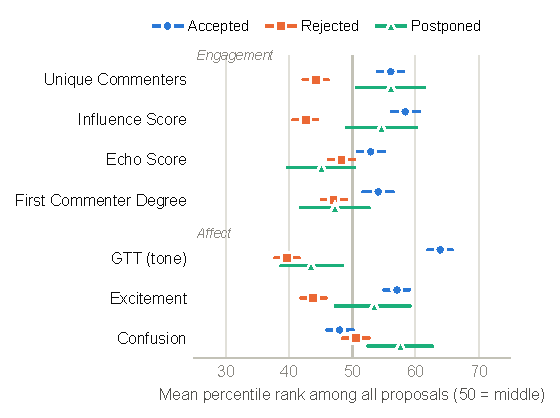
\includegraphics[width=\columnwidth]{figures/fig_outcome_profile.pdf}
\caption{Outcome profiles. For each metric, every proposal's percentile rank among all 1,469 proposals, averaged per outcome group (markers), with 95\% bootstrap intervals (lines); 50 is the middle of all proposals. Postponed proposals sit with accepted ones on engagement, with rejected ones on Echo Score, First Commenter Degree, and GTT, and above both on confusion.}
\label{fig:profile}
\end{figure}

\textbf{Postponed Proposals:} Taken together, postponed proposals combine features of both other groups, as Figure~\ref{fig:profile} shows. On engagement they resemble accepted proposals, with as many unique commenters and comments and as high an Influence Score, and exceed rejected proposals ($r = 0.234$--$0.238$); fewer of their commenters, however, belong to the governance core ($r = 0.167$ vs.\ accepted), as in rejected proposals. On tone they resemble rejected proposals, and their discussions carry the most confusion, disappointment, and embarrassment of the three groups, alongside the enthusiasm of accepted ones.

\begin{tcolorbox}[
  colback=heatmaplight,
  colframe=heatmapdark,
  coltitle=white,
  fonttitle=\bfseries,
  title=Summary --- RQ1
]
Accepted proposals drew broader participation (Mdn\,=\,11 vs.\ 8 unique commenters, $r = 0.237$), higher-centrality commenters ($r = 0.316$), and a less negative tone (GTT $r = 0.481$) than rejected ones; all three survive the within-author comparison, GTT most robustly ($r = 0.738$; time-matched $r = 0.599$). Postponed proposals are engaged like accepted ones but with fewer governance-core members, toned like rejected ones, and carry the most confusion ($r = 0.201$ vs.\ accepted).
\end{tcolorbox}

\subsection{RQ$_2$: Early Visibility}
\label{sec:rq2}
\begin{figure}[t]
\centering
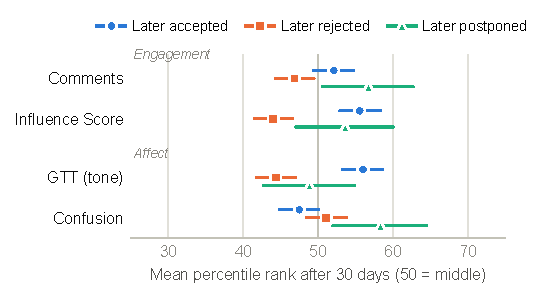
\includegraphics[width=\columnwidth]{figures/fig_early_window.pdf}
\caption{Early visibility. Proposals still undecided 30 days after submission (430 later accepted, 442 later rejected, 73 later postponed), measured over their first 30 days of comments. Markers show each group's mean percentile rank among these proposals, with 95\% bootstrap intervals. Proposals that will be postponed already have as much discussion and influence as those that will be accepted, and more than those that will be rejected, and they carry the most confusion; confusion barely separates proposals that will be accepted from those that will be rejected.}
\label{fig:early}
\end{figure}

Table~\ref{tab:early} reports the comparisons among proposals still undecided at day 30 and day 60, and Figure~\ref{fig:early} shows the day-30 profile. At day 30, the proposals that will later be postponed already have more discussion than later-rejected proposals (Mdn\,=\,21 vs.\ 14 comments; $p = 0.022$, $r = 0.199$) and a higher Influence Score (Mdn\,=\,517 vs.\ 357; $p = 0.022$, $r = 0.195$), at the level of later-accepted proposals (Mdn\,=\,17 comments; Influence Score 539.5). They also carry the most confusion (Mdn\,=\,0.156, vs.\ 0.122 for later-accepted and 0.133 for later-rejected proposals), significantly more than later-accepted proposals ($p = 0.015$, $r = 0.219$); the difference from later-rejected proposals is not significant ($p = 0.098$, $r = 0.144$). At the same point, confusion does not separate later-accepted from later-rejected proposals ($p = 0.113$, $r = 0.071$), while GTT ($r = 0.232$), Influence Score ($r = 0.231$), and excitement ($r = 0.174$) do. Echo Score does not separate postponed proposals from either group in either window.

\vspace{-10pt}
\begin{table}[h]
\centering
\caption{Proposals still undecided at day 30 and day 60, measured over the comments posted so far. Bold: $p < 0.05$ after Benjamini--Hochberg adjustment within each window.}
\label{tab:early}
\resizebox{\columnwidth}{!}{%
\begin{tabular}{lrrrrrr}
\toprule
\textbf{Metric}
  & \textbf{Acc Mdn}
  & \textbf{Rej Mdn}
  & \textbf{Pst Mdn}
  & \textbf{A/R $r$}
  & \textbf{A/P $r$}
  & \textbf{R/P $r$} \\
\midrule
\multicolumn{7}{l}{\textit{Day 30 ($n$ = 430/442/73):}} \\
Comments           & 17 & 14 & 21
  & \textbf{0.105} & 0.091 & \textbf{0.199} \\
Unique Commenters  & 8 & 7 & 8
  & \textbf{0.091} & 0.051 & 0.141 \\
Influence Score    & 539.5 & 357 & 517
  & \textbf{0.231} & 0.041 & \textbf{0.195} \\
Echo Score         & 0.167 & 0.125 & 0.125
  & \textbf{0.096} & 0.137 & 0.035 \\
GTT                & $$-$$0.117 & $$-$$0.267 & $$-$$0.231
  & \textbf{0.232} & 0.152 & 0.099 \\
Excitement         & .00088 & .00067 & .00072
  & \textbf{0.174} & 0.082 & 0.087 \\
Confusion          & .12156 & .13316 & .15597
  & 0.071 & \textbf{0.219} & 0.144 \\
\midrule
\multicolumn{7}{l}{\textit{Day 60 ($n$ = 291/352/64):}} \\
Comments           & 21 & 16 & 27.5
  & \textbf{0.176} & 0.062 & \textbf{0.241} \\
Unique Commenters  & 9 & 8 & 10
  & \textbf{0.154} & 0.021 & 0.178 \\
Influence Score    & 658 & 395.5 & 646
  & \textbf{0.281} & 0.008 & \textbf{0.294} \\
Echo Score         & 0.143 & 0.125 & 0.118
  & 0.046 & 0.100 & 0.040 \\
GTT                & $$-$$0.139 & $$-$$0.234 & $$-$$0.249
  & \textbf{0.165} & 0.151 & 0.023 \\
Excitement         & .00096 & .00071 & .00087
  & \textbf{0.186} & 0.071 & 0.101 \\
Confusion          & .12990 & .13316 & .14710
  & 0.029 & 0.175 & 0.132 \\
\bottomrule
\end{tabular}%
}
\end{table}

At day 60, engagement separates later-postponed from later-rejected proposals more strongly (Influence Score $p = 0.001$, $r = 0.294$), whereas the confusion differences are of similar size ($r = 0.132$--$0.175$) but not significant after adjustment. The same-cohort check shows that the day-60 pattern was already present at day 30: for proposals still undecided at day 60, their day-30 comments already separate later-postponed from later-rejected proposals on Influence Score ($p = 0.007$, $r = 0.269$) and comments ($p = 0.010$, $r = 0.246$). Waiting longer adds little.

\begin{tcolorbox}[
  colback=heatmaplight,
  colframe=heatmapdark,
  coltitle=white,
  fonttitle=\bfseries,
  title=Summary --- RQ2
]
Within 30 days, proposals that will be postponed already attract more engagement than those that will be rejected (Influence Score $r = 0.195$) and more confusion than those that will be accepted ($r = 0.219$). At that point confusion does not separate eventual acceptance from rejection ($r = 0.071$), so it signals stalling rather than failure.
\end{tcolorbox}

\section{Discussion}
\textbf{Governance debt is distinct from rejection.} Rejected proposals draw comparatively little participation, few established participants, and a negative tone. Postponed proposals draw as much participation as accepted ones, from participants who are as established on average, yet do not converge: their tone stays negative and their discussions carry more confusion than accepted ones. They also involve fewer members of the governance core, the participants who most often carry proposals to a decision, although this difference is not visible in the early windows. This is the state we call governance debt. The community pays the cost of deliberation without obtaining a decision, and the cost is carried forward with the proposal. The two failure modes call for different responses. A rejected proposal may need a better design; a stalling one may need less debate and more clarification, for instance a summary of the open questions, an explicit statement of what would settle them, or a dedicated design meeting. Rust's RFC template already asks authors to list unresolved questions; governance debt may arise when such questions accumulate in the discussion faster than they are consolidated.

\textbf{An early signal, not a predictor.} The effects in RQ$_2$ are small ($r \approx 0.2$) and should not be read as a classifier. They suggest a triage heuristic: a proposal that, a month after submission, draws unusually active and established participation together with unusually high confusion deserves a maintainer's attention. Because, at that stage, confusion barely separates eventual acceptance from rejection ($r = 0.071$), it points to a stalling discussion rather than a weak proposal.

\textbf{Tone is the most robust correlate of acceptance.} GTT separates accepted from rejected proposals more than any engagement metric, and it survives both within-author designs, including proposals by the same author submitted about two months apart. Unique Commenters and Influence Score also survive the author-median comparison, in line with pull-request studies showing that social factors shape acceptance~\cite{tsay2014influence}, but weaken when an author's proposals are paired in time, suggesting that part of the engagement gap reflects an author's changing standing. We cannot tell whether tone reflects the community's reaction to proposal quality or shapes the outcome; either way, it is the most consistent process signal we observed.

\section{Threats to Validity}
\textbf{Construct validity.} SiEBERT has only positive and negative classes, so a neutral technical comment must be classified as one or the other; 96\% of comments receive a score beyond $\pm 0.9$, and GTT mostly reflects the balance of positive and negative classifications. To test whether this matters, we re-scored all comments with a three-class model that allows neutral comments (\texttt{cardiffnlp/twitter-roberta-base-sentiment-latest}). GTT computed from this model gives the same picture with somewhat smaller effects, all significant: accepted vs.\ rejected $r = 0.378$ (SiEBERT: 0.481), accepted vs.\ postponed $r = 0.325$ (0.440), within the same author $r = 0.697$ (0.738; time-matched 0.474 vs.\ 0.599), and at day 30 $r = 0.174$ (0.232). The GTT results therefore do not depend on forcing neutral comments into a polarity. The GoEmotions model was trained on Reddit comments and has not been validated on technical discussion; in particular, \emph{confusion} may partly capture ordinary technical questions. Because SE-specific tools perform better on technical text~\cite{novielli2019sentiment, islam2018sentistrength}, manually validating the emotion labels on a sample of RFC comments is an important next step. Engagement measures are proxies: prospective degree counts participation, not authority or expertise, and degree is necessarily low for the earliest proposals. Echo Score depends on the core size; we follow the median rule ($k = 10$), and other choices may change its values.

\textbf{Internal validity.} Outcome labels depend on repository labels; we excluded proposals whose labels are inconsistent with their outcome. We analyze each proposal's whole discussion, including comments posted during the formal decision process and after the merge or close; some differences, particularly in tone, may therefore partly reflect the decision itself rather than precede it. RQ$_2$ addresses this by analyzing only the early comments of proposals that were still undecided. The within-author comparisons hold author identity constant but not proposal quality, and comparisons involving postponed proposals rest on 40--61 authors. We report associations, not causal effects, and adjust for multiple comparisons within each table.

\textbf{External validity.} We study a single process and aim for analytical rather than statistical generalization~\cite{yin2009case}. We expect the distinction between rejection and postponement to transfer to formal deliberative processes such as PEPs, KEPs, and Swift Evolution, but not necessarily to informal or single-maintainer projects.

\section{Conclusion}
Analyzing 1,469 Rust RFCs, we find that postponement is a distinct outcome of deliberation: postponed proposals draw participation like accepted ones, tone like rejected ones, and the most confusion of all. We call this state governance debt and show that part of its signature is visible within 30 days. We also find that discussion tone is the most robust correlate of acceptance, surviving within-author comparisons in which engagement differences weaken. Future work will validate the emotion measures manually, replicate the analysis in other proposal processes such as PEPs and KEPs, and work with maintainers to test whether early signals of governance debt help them intervene.

\section*{Data Availability}
Our data, analysis scripts, and results are available in the replication package~\cite{rrgc2026}.

\bibliography{references}

\end{document}
\endinput
